\documentclass[12pt]{article}

\usepackage[utf8]{inputenc}
\usepackage{listings}
\usepackage{graphicx}
\usepackage{float}
\usepackage{geometry}
\usepackage{authblk}
\usepackage{setspace}

\newcommand*{\TitleFont}{
  \usefont{\encodingdefault}{\rmdefault}{b}{n}
  \fontsize{30}{40}
  \selectfont}

\usepackage{parskip}
\setlength{\parskip}{1.0\baselineskip plus2pt minus2pt}
%% \setlength{\baselineskip}{1cm}

\addtolength{\topmargin}{-50pt}
\addtolength{\textheight}{130pt}
\addtolength{\textwidth}{95pt}
\addtolength{\oddsidemargin}{-45pt}

\title{\TitleFont{Computação Gráfica}}
\author{David Gomes (2013136061) \and \vspace{-0.1cm} André Baptista (2012137523)}
\date{}

\begin{document}
\maketitle

\section*{Introdução}
O nosso projeto de Computação Gráfica consiste num ambiente 3D com várias bolas a movimentar-se
dentro de um cubo coberto, na sua base, por água.

\begin{figure}[H]
  \centering
  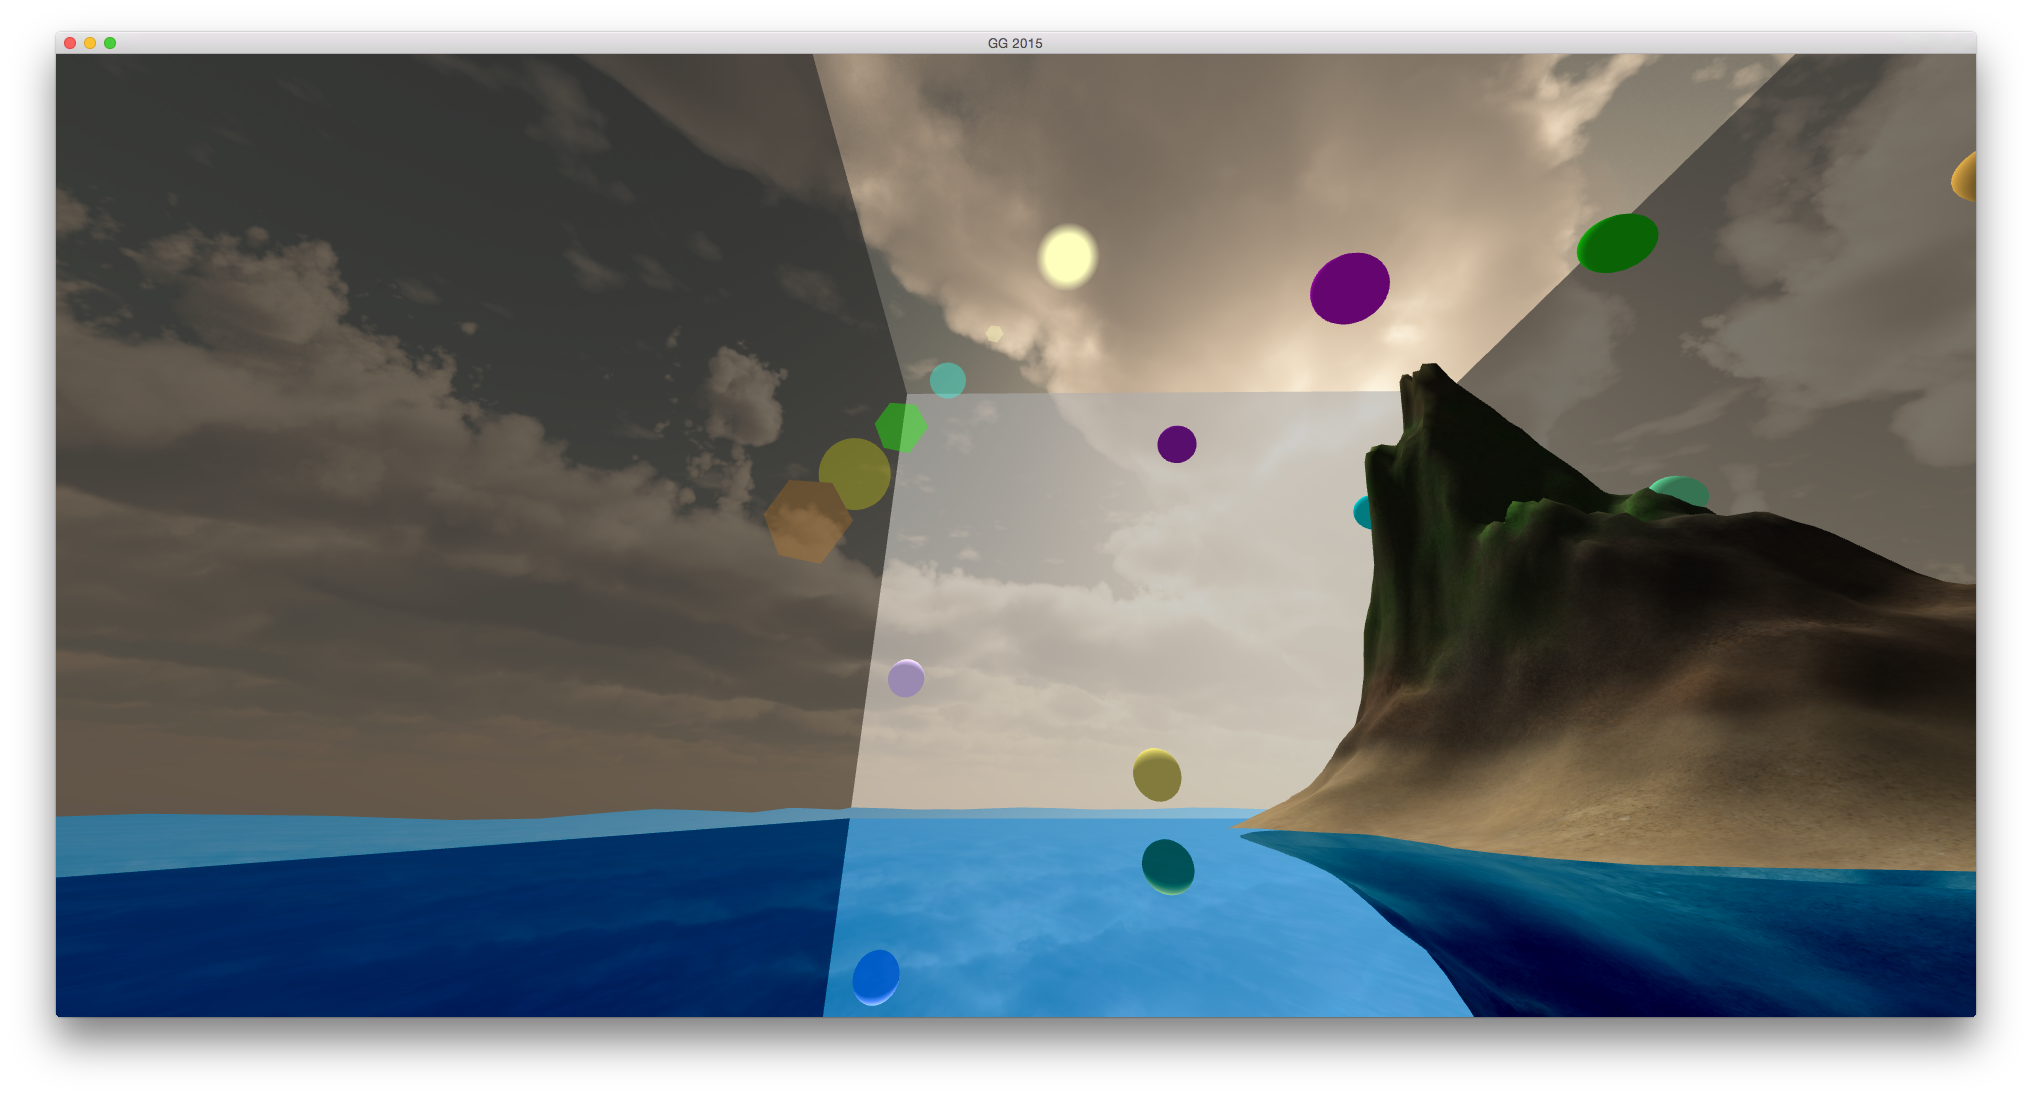
\includegraphics[width=0.75\textwidth]{screenshot}
\end{figure}

O objetivo deste relatório é apresentar algumas das \textit{features} do nosso projeto e explicar sucintamente a sua implementação.

\pagebreak

\subsection*{\textit{Object Loader}}
Para facilitar o desenvolvimento do projeto criámos um \textit{loader} de objetos que desenha modelos
a partir de ficheiros \texttt{.obj}. Com este mecanismo associado à classe \texttt{Object}, carregamos o modelo da ilha assim como o do cubo. Foi também criado um loader de texturas, que permite desenhar automaticamente as texturas nos objectos, recorrendo aos UVs definidos nos ficheiros \texttt{.obj} correspondentes. Esta funcionalidade permite carregar para a cena objectos desenhados previamente em software gráfico 3D, como por exemplo o Blender, que por sua vez torna possível que estes sejam modelados e pintados facilmente.

\subsection*{\textit{Shaders}}
Durante o desenvolvimento do projecto, procurámos explorar \textit{pipeline} programável, recorrendo a shaders \texttt{GLSL}. Foram implementados tanto \textit{vertex shaders} como \textit{fragment shaders}, como irá ser descrito nas próximas \textit{features}. Foram utilizadas as variáveis \textit{uniform} e \textit{varying}, para permitir enviar informação do programa principal para o \textit{shader} e partilhar informação entre os \textit{vertex shaders} e os \textit{fragment shaders}, respectivamente.

\subsection*{Sol}
O sol é uma uma fonte de luz direccional e um pequeno círculo que é desenhado utilizando as primitivas básicas do OPENGL, mas alterado ao nível do pixel através de um \textit{fragment shader}. Este \textit{shader} tem acesso às coordenadas do píxel actual, o que nos permite calcular a distância até ao centro do círculo e, por conseguinte, calcular variações de transparência e de cor. Foi também implementado um \textit{day-night cycle} que faz com que a cor do sol também varie de acordo com a sua posição ao longo do dia. Para tornar esta funcionalidade possível foi criada uma variavél \textit{uniform} que contém informação sobre a posição actual do sol.

\subsection*{\textit{Skybox}}
Foi implementada uma \textit{Skybox} que é constituída por um cubo que envolve o mundo, cujas faces interiores têm uma textura que permite simular o céu. Devido à existência do \textit{day-night cycle}, o brilho do céu também varia de acordo com a posição do sol.

\subsection*{\textit{Lens Flare}}
Foi também implementado um efeito de \textit{lens flare}, que varia de acordo com a orientação do observador e a posição do sol. Isto é, se o observador olhar para o sol directamente é possível observar um efeito provocado pela luz do mesmo. Para implementar este efeito, que é bastante comum em jogos de computador, foi necessário recorrer às matrizes \textit{modelview}, \textit{projection} e \textit{viewport}. Estas matrizes foram utilizadas como argumento da função \texttt{gluProject}, que permite obter as coordenadas 2D do ecrã de um objecto do mundo 3D. De seguida a projecção é alterada para o modo ortogonal (projecção pararela) para facilitar o desenho deste efeito, que é constituído por círculos e hexágonos, cujas cores são alteradas utilizando um \textit{fragment shader}. Este \textit{shader} tem acesso ao índice do polígono actual e a posição do sol, que permite variar a transparência e a cor do efeito.

\subsection*{Água}
A água é uma grelha de planos, cujos vértices são manipulados por um \textit{vertex shader}. A altura de cada vértice é alterado através de funções sinusoidais que simulam ondas do mar, de acordo com o período e amplitude da onda. As cores de cada pixel são processadas através de um \textit{fragment shader} que será descrito no ponto seguinte.

\subsection*{Reflexão}
Para simular a reflexão da água, a cena é renderizada duas vezes. A primeira renderização é invertida no eixo dos \textit{yy} e é feita utilizando a função \texttt{glClipPlane}, que permite desenhar apenas os objectos que se encontram numa posição superior ao nível da água. De seguida é gerada uma imagem 2D que é guardada numa textura, recorrendo à função \texttt{glCopyTexSubImage2D}. A água é constituída por uma textura própria que simula a sua superfície e pela textura da reflexão. Estas duas texturas são posteriormente utilizadas pelo \textit{fragment shader} para calcular a cor. Este \textit{shader} realiza uma mistura de cores entre: cor base, textura base, textura reflectida e componente especular da reflexão do sol. A textura reflectida é deformada de acordo com a amplitude actual da onda e a reflexão do sol é calculada tendo em conta a posição do observador. A cor da reflexão do sol é ainda influenciada pela posição do sol, de modo a simular o pôr do sol.

\subsection*{Colisões}
Vários tipos de colisões simples são usadas no nosso projeto, seja para detetar colisão entre duas esferas ou entre esferas e planos.

\subsection*{Explosões (partículas)}
Implementamos um efeito de partículas que gera centenas de partículas (implementadas com pequenos cubos tridimensionais de OpenGL) para simular uma explosão fogosa quando duas bolas colidem.

\subsection*{Lançamento de Bolas}
Ao carregarmos com o rato esquerdo no ecrã será "atirada" para a cena uma nova bola com a direção
do observador que, tal como qualquer outra bola, interage com as restantes (podendo portanto colidir com qualquer coisa).

\end{document}